\documentclass[prb,aps,nobibnotes,twocolumn,doublespace,twocolumngrid,superbib]{revtex4}
%\documentclass[prb,aps,nobibnotes,superbib,preprint]{revtex4}

\usepackage{graphicx}
\usepackage{amsfonts}
\usepackage{amsmath}
\usepackage{bm}
\usepackage{alltt}
\usepackage{dcolumn} 
\usepackage{graphicx}
\makeatletter 
\makeatother

\begin{document}

\title{Linear scaling computation of the Fock matrix. VIII. \\ 
       Periodic, exact exchange in the $\Gamma$-point approximation. }

\author{C. J. Tymczak}
\author{Valery Weber}
\author{Eric Schwegler}
\author{Matt Challacombe}

\affiliation{Theoretical Division, Los Alamos National Laboratory, Los Alamos,
New Mexico 87545 }

\affiliation{Larance Livermore}


\date{\today}
\begin{abstract}
A translationally invariant formulation of the Hartree-Fock (HF) $\Gamma$-point approximation
is presented.   This formulation is achieved through introduction of  the  Minimum Image Convention (MIC) at 
the level of primitive two-electron integrals, and implemented in a periodic version of the 
ONX algorithm [J.~Chem.~Phys, {\bf 106} 9708 (1997)] for linear scaling computation of the
exchange matrix. Convergence of the HF-MIC $\Gamma$-point model to the HF ${\bf k}$-space limit 
is demonstrated for fully periodic magnesium oxide, ice and diamond.  Computation of the diamond
lattice constant using the HF-MIC model together with the hybrid PBE0 density functional 
[Theochem, {\bf 499} 145 (1999)], yeilds $a_0=3.569$ with the 6-21G* basis set and a 
$3\times3\times3$ supercell.  Linear scaling computation of the HF-MIC exchange matrix is demonstrated 
for diamond and ice in the condensed phase. 
\end{abstract}

\pacs{}

\maketitle

\footnotetext[1]{\tt tymczak@lanl.gov}
%\footnotetext[2]{\tt vweber@lanl.gov}
%\footnotetext[3]{\tt schwegler@llnl.gov}
%\footnotetext[4]{\tt mchalla@lanl.gov}
\footnotetext[5]{\tt Preprint LA-UR 03-9043}

\section{INTRODUCTION}

In a preceeding companion article \cite{CTymczak04A},  methods were introduced for constructing 
the periodic Coulomb and Exchange-Correlation matrix in the $\Gamma$-point approximation that 
achieve  a cost  scaling only linearly with system size, $N$.  In this paper, an $N$-scaling 
algorithm is presented for computation of the periodic Hartree-Fock (HF) exchange matrix in the 
$\Gamma$-point limit.   The Hartree-Fock approximation is often a fast, first 
approximation and also a starting point for correlated ``wavefunction'' methods.  
Also, the hybrid Hartree-Fock/Density Functional Theory (HF/DFT) model chemistries are an important next 
in step in accuracy beyond the pure Generalized Gradient Approximation \cite{Gill92,Becke93,VBarone96,CAdamo99}.
Together with linear scaling methods for computing the density matrix \cite{ANiklasson02A,ANiklasson03}, these 
advances provide a framework for the application of both HF and HF/DFT models to large condensed 
phase systems, surfaces and wires.   

To date, condensed phase HF and HF/DFT calculations have been carried out almost 
exclusively with the {\em ab initio} solid state program {\sc CRYSTAL} \cite{RDovesi00}, 
which employs conventional (non-direct) ${\cal O}(N^4)$ algorithms for evaluation of the 
HF exchange matrix.  The {\sc CRYSTAL} program employs methods for ${\bf k}$-space integration, 
which generate wavefunctions with the correct translational symmetries.   While the  
$\Gamma$-point approximation forgoes ${\bf k}$-space integration, it does recover the correct 
symmetries in the limit of a large super-cell.  With a more tractable formulation and asymptotic 
correctness in the limit of large systems,  the $\Gamma$-point  approximation would seem an 
ideal basis for linear scaling exchange algorithms.   However in preliminary studies, we found 
that the naive HF $\Gamma$-point approximation converged to position dependent values, and that 
even in the large super-cell limit,  values different from the ${\bf k}$-space integration limit were approached.

In this paper we develop a translationally invariant definition of $\Gamma$-point 
Hartree-Fock exchange, which correctly approaches the ${\bf k}$-space integration value
in the limit of a large super-cell.  This is accomplished through introducing a Minimum 
Image Convention (MIC) into the exchange kernel at the level of primitive two-electron integrals,  
as described in Section \ref{gammapoint}.  Incorporation of the MIC integrals into a periodic 
version of the {\sc ONX} algorithm \cite{ESchwegler97} for linear-scaling computation of the HF 
exchange matrix is then described in Section \ref{implementation}.  In Section \ref{validation} 
we demonstrate convergence of the HF-MIC model chemistry to the $\bf k$-space integration 
limit for a number of systems, and in Section \ref{scaling} we demonstrate linear scaling
for both diamond and ice.  In Section \ref{discussion} we discuss these results,
and then in Section \ref{conclusions} we sumarize our results.

%%%%%%%%%%%%%%%%%%%%%%%%%%%%%%%%%%%%%%%%%%%%%%%%%%%%%%%%%%%%%%%%%%%%%%%%%%%%%%%
%\newpage
%%%%%%%%%%%%%%%%%%%%%%%%%%%%%%%%%%%%%%%%%%%%%%%%%%%%%%%%%%%%%%%%%%%%%%%%%%%%%%%

\section{Periodic exact exchange}

In the conventional implementations of periodic boundary conditions, the 
Bloch functions 
\begin{equation}
\psi^{\bf k}_a({\bf r})  =  \sum_{\bf R} e^{i {\bf k}\cdot {\bf R}} \phi_a ({\bf r}-{\bf R}),
\label{Block}
\end{equation}
are often constructed from non-orthogonal functions local to the unit cell (UC). Here, the 
local function
$\phi_a$ is a Gaussian-Type Atomic Orbital (GTAO) centered on atom {\bf A}, while the 
sum on {\bf R} runs over the Bravais lattice defined by integer translates of the primitive 
lattice vectors {\bf a}, {\bf b} and {\bf  c}.  Inversely, the vector {\bf k} runs over 
the reciprocal Bravais lattice vectors.

To date, rapid computation of the Hartree-Fock exchange interaction demands
the analytic evaluation of two-electron integrals, which is possible when the 
local basis functions are of Cartesian Gaussian type.  
Typically, these functions have the form
\begin{equation}
\phi_a ({\bf r}) = (x-A_x)^{l_a} (y-A_y)^{m_a} (z-A_z)^{n_a}{\large e}^{-\zeta_a ({\bf r}-{\bf A})^2}
\end{equation}
where the triad $\{l_a,m_a,n_a\}$ sets angular symmetry  
and the exponent $\zeta_a$ is chosen to describe a particular length scale. 
Gaussian basis functions are often contracted to approximate 
atomic eigenfunctions \cite{}.
 
With periodic boundary conditions, the exact {\bf k}-dependent Hartree-Fock exchange matrix is 
\cite{RDovesi00,MCausa88}
\begin{equation}
K_{ab} [{\bf k}] = \sum_{{\bf G}} K_{ab} [{\bf G}] e^{i {\bf k}\cdot {\bf G}} \, ,
\label{Kinkspace}
\end{equation}
where
\begin{equation}
K_{ab} [{\bf G}] = - \frac{1}{2}
\sum _{{\bf H N},c d} P_{cd}[{\bf N}]
\left(
      \phi        _a    
      \phi^{\bf H}_c    
{\big | }
      \phi^{\bf G}_b    
      \phi^{\bf H+N}_d  
\right) 
\label{CryEq}
\end{equation}
is defined in real space, and the two-electron integrals, written in the chemist notation, are 
\begin{eqnarray}
\left(
      \phi        _a  
      \phi^{\bf H}_c  
{\big | }
      \phi^{\bf G}_b  
      \phi^{\bf H+N}_d
\right)
= \quad\quad\quad\quad\quad 
 \quad\quad\quad\quad\quad  
 \quad\quad\quad\quad\quad 
\nonumber \\
\iint d {\bf r} d {\bf r}'
\frac{{\phi_a({\bf r}) \phi_c({\bf r}+{\bf H}})\phi_b({\bf r'}+{\bf G})\phi_d({\bf r'}+{\bf H}+{\bf{N})}}
{{\left|{\bf r}-{\bf r'}\right|}} \, .
\nonumber\\
\end{eqnarray}

The formally infinite sums over lattice vectors in Eq.~(\ref{CryEq}) involve 
many contributions that are in practice infinitesimal.  In part this is due to 
the decay between local basis function products $\phi_a \phi_c $; the product of
two Guassians centered at ${\bf A}$ and ${\bf C}$ decays also as a Gaussian with 
$|{\bf A}-{\bf C}|$. 
Truncation based purely on the overlap of Gaussian basis functions is reliable and
well controlled, leading  to ${\cal O}(N)$ product terms.
Additionally, the density matrix is known to decay exponentially 
for non-metallic systems.  A radial cutoff defining the range of allowed exchange 
interactions may be used to exploit this fall off {\em a priori} by confining summation over 
${\bf N}$ \cite{RDovesi00,MCausa88,REuwema74,CPisani80,RDovesi80} to only those terms that 
satisfy the imposed geometric constraints.  Methods equivalent to the radial cutoff have also 
been used to achieve $N$-scaling of the exchange matrix in gas phase calculations, which set
a maximal range allowed between atom-atom pairs $\bf C$ and $\bf D$ that 
address elements of the density matrix $P_{cd}$ \cite{ESchwegler96,JBurant96}.  

%%%%%%%%%%%%%%%%%%%%%%%%%%%%%%%%%%%%%%%%%%%%%%%%%%%%%%%%%%%%%%%%%%%%%%%%%%%%%%%
%\newpage
%%%%%%%%%%%%%%%%%%%%%%%%%%%%%%%%%%%%%%%%%%%%%%%%%%%%%%%%%%%%%%%%%%%%%%%%%%%%%%%

\section{Exchange at the $\Gamma$-point}\label{gammapoint}

The $\Gamma$-point approximation limits {\bf k}-space sampling to just the central cell at
${\bf k} = 0$.   In the naive $\Gamma$-point limit, we take ${\bf P[ N ] } \equiv \delta_{\bf N,0} \, {\bf P} $,
reducing Eq.~(\ref{CryEq}) to the less cumbersome relation (note, we have re-labled the lattice sums 
for simplicity):
\begin{equation}
K_{ab}=
\sum _{{\bf H G}, c d} P_{cd}
\left(
      \phi_a    
      \phi^{\bf H}_c    
{\big | }
      \phi_b  
      \phi^{\bf G}_d  
\right)\, .
\label{CryEq_2}
\end{equation}
However, there are significant problems with this naive model,  as  the exact exchange potential, 
symmetric in the limit of infinite summation, has been truncated asymetrically.
This truncation leads to an energy expression 
\begin{equation}
E_x[{\bf P}^a,{\bf P}^b] = {\rm Tr} \left[  {\bf P}^a \cdot {\bf K}^b  \right] \, ,
\end{equation}
which violates permutational symetry of the exchange kernel; that is, in general, 
$E_x[{\bf P}^a,{\bf P}^b] \ne E_x[{\bf P}^b,{\bf P}^a]$.   

A more serious deffect of  Eq.~\ref{CryEq_2} is that $E_x$  varies with position of the coordinates.  
This translational variance has a well understood analogue in classical molecular dynamics 
\cite{NMetropolis53,MAllen90,MHloucha98}, where the arbitrary truncation of short range potentials also leads 
to numerical artifacts in energies and forces.  In both cases, translational invariance is  restored by introducing the Minimum Image Convention (MIC), 
which ensures that the distance between neighboring images is always used in computing interactions. 
In computation of the Hartree-Fock exchange matrix, the MIC $\Gamma$-point approximation is just
\begin{equation}
K_{ab}=
\sum _{{\bf H G} c d} P_{cd}
\left(
      \phi        _a    
      \phi^{\bf H}_c    
{\big | }
      \phi        _b    
      \phi^{\bf G}_d  
\right)_{\rm  MIC},
\label{MIC}
\end{equation}
where the MIC condition is applied in computation of the two electron integrals
at the contraction phase, ensuring that primitive charge distributions 
interact consistently over a minimum distance.  In particular, if the primitive basis 
function product $\phi_a \phi^{\bf H}_c$ is centered at ${\bf P}$ and the primitive product 
$\phi_b \phi^{\bf G}_d$ is at ${\bf Q}$, then the minimum image convention is 
applied to the interaction vector ${\bf PQ} \equiv {\bf P}-{\bf Q}$ using
\begin{subequations}
\begin{eqnarray}
{\bf pq}&=&{\bf M}^{-1} \cdot {\bf PQ} \\
pq_i & =& pq_i - {\tt ANINT} \left( pq_i -{\tt SIGN}\left( \delta,pq_i\right) \right) \\
{\bf PQ}_{\rm MIC}&=&{\bf M} \cdot {\bf pq} 
\end{eqnarray}
\end{subequations}
where $\delta \approx 10^{-15}$ and is needed to avoid wrapping errors \footnote{
This numerical $\delta$ is required to yeild a consistent wrapping when distributions lie 
exactly at the cell boundary.  In effect, this implementation changes the wrapping condition
from $|pq_i| \ge 1$ to $|pq_i| > 1$.},   and 
${\bf  M}$ is the $3 \times 3$ shape matrix of the unit cell, 
composed of the primative lattice vectors,
\begin{equation}
{\bf M} = \left( {\bf a}:{\bf b}:{\bf c} \right)
\end{equation}
This approach is completely general, and can be used at the primitive level with any modern approach
to computing two-electron integrals. Imposing this condition recovers translational invariace of the
exchange matrix. However, the MIC condition does not recover the Exchange Kernel Permutational Symmetry 
(EKPS).  With greater expense, we could recover the EKPS by  explicitly sysmmetrizing the primitive Gaussian 
products within the kernel.  However, in the limit of large systems, where the range of the density 
matrix becomes smaller then the system size the  EKPS is recovered as demonstrated in Section \ref{validation}.

\section{Optimial damping and symmetry of the exchange kernel}

For difficult, unstable SCF problems, the Optinal Damping Algorithm (ODA) of Cances \cite{ECances00} is
an efficient method that gaurantees convergence of the HF model.  
However,  permutational symmetry of the exchange kernel is an implicit, simplifying assumption in formulation
of the conventional ODA algorithm.   For small periodic systems, violation of the EKPS creates problems
for the ODA, leading to a non-quadratic behavior (the HF model should yeild an exactly quadratic, convex 
minimization problem).   While the EKPS is restored with increasing system size, loose numerical thresholds
in the linear scaling algorithms can also lead to loss of the EKPS in the limit of a large system.  
In both cases, loss of EKPS can lead to incorrect determination of the ODA mixing parameter
%
\begin{eqnarray}
\lambda = {{\frac{d E^0}{d \lambda}} \over {3E^1-3E^0-2{\frac{d E^0}{d \lambda}}-{\frac{d E^1}{d \lambda}}}}
\end{eqnarray}
%
where the superscripts indicate consecutive steps in the SCF cycle given by the endpoints, 
with $\lambda \in [0,1]$.   It is of course a simple matter to reformulate the ODA, using definitions 
for the endpoint derivatives that do not assume EKPS:
\begin{eqnarray}
%E[0] &&= {\rm Tr}\left[{\bf P}_0 \left({\bf T} + {\bf F}_0 \right)\right]+E^{0}_{\rm ne} \nonumber\\
%E[1] &&= {\rm Tr}\left[{\bf P}_1 \left({\bf T} + {\bf F}_1 \right)\right]+E^{1}_{\rm ne} \nonumber\\
\frac{d E^0}{d \lambda} &&=  E^{1}_{\rm ne}-E^{0}_{\rm ne}  
+{\rm Tr}\left[\left( {\bf P}^1 - {\bf P}^0 \right) {\bf T}  \right]\nonumber\\
&& +{\rm Tr}\left[ {\bf P}^1 {\bf F}^0 \right] 
   +{\rm Tr}\left[ {\bf P}^0 {\bf F}^1 \right] 
   -2 {\rm Tr}\left[ {\bf P}^0 {\bf F}^0 \right] \nonumber\\
\frac{d E^1}{d \lambda} &&=  E^{1}_{\rm ne}-E^{0}_{\rm ne}  
+{\rm Tr}\left[\left( {\bf P}^1 - {\bf P}^0 \right) {\bf T}  \right]\nonumber\\
&& -{\rm Tr}\left[ {\bf P}^1 {\bf F}^0 \right] 
   -{\rm Tr}\left[ {\bf P}^0 {\bf F}^1 \right] 
   +2 {\rm Tr}\left[ {\bf P}^1 {\bf F}^1 \right] \, , \nonumber\\
\end{eqnarray}
where  ${\bf F}$ is the Fockian, $\bf T$ is the kinetic energy matrix  and $E_{\rm ne}$ is the nuclear-electrostatic energy.
This  modified ODA leads to the correct quadratic parameterization and guarantees convergence of the HF-MIC model.  

%%%%%%%%%%%%%%%%%%%%%%%%%%%%%%%%%%%%%%%%%%%%%%%%%%%%%%%%%%%%%%%%%%%%%%%%%%%%%%%
%\newpage
%%%%%%%%%%%%%%%%%%%%%%%%%%%%%%%%%%%%%%%%%%%%%%%%%%%%%%%%%%%%%%%%%%%%%%%%%%%%%%%

\section{Implementation}\label{implementation}

A general treatment of $\Gamma$-point Periodic Boundary Conditions has been implemented in the MondoSCF
suite of programs for linear scaling quantum chemistry.  A detailed account of these developments for 
pure Density Functional Theory has been given in a companion paper \cite{CTymczak04A}, including the periodic 
development of the Quantum Chemical Tree Code ({\sc QCTC}) for performing $N$-scaling Coulomb summation.  

The Order N eXchange ({\sc ONX}) algorithm \cite{ESchwegler97} for computing the gas phase exchange matrix 
has been modified by placing dual loops running over the lattice vectors 
${\bf H}$ and ${\bf G}$ around the original ONX loop structures.  Two ordered bra and ket distribution 
buffers are assembled for each lattice vector pair, which are then used to drive the basic {\sc ONX} algorithm.
The Minimum Image Convention has been introduced into the primitive contraction stage, in the 
Vertical Recurrence Relations component of a symmetry driven Head-Gordon Pople \cite{MHeadgordon88} scheme for 
computing two-electron integrals.  While this implementation is linear scaling and simple, it suffers 
from a number of drawbacks that we will set forth in detail shortly, together with a more efficient 
algorithm able to achieve scalable parallelism \cite{}.

%%%%%%%%%%%%%%%%%%%%%%%%%%%%%%%%%%%%%%%%%%%%%%%%%%%%%%%%%%%%%%%%%%%%%%%%%%%%%%%
%\newpage
%%%%%%%%%%%%%%%%%%%%%%%%%%%%%%%%%%%%%%%%%%%%%%%%%%%%%%%%%%%%%%%%%%%%%%%%%%%%%%%

\begin{table}[ht]
\caption{Progression of Hartree-Fock $\Gamma$-point super-cell calculations 
for MgO using the periodic RHF-MIC and RHF 8-511G/8-51G level of theory.  Comparison is 
made to a final value approaching the ${\bf k}$-space integration limit for the primitive cell.}
\label{MgOTable}
\center{\begin{tabular}{lrll}
\toprule
Program         & $N_{\rm at}$              & Energy (au)    & Energy/$N_{\rm at}$\\ 
\colrule
%{\sc MondoSCF}       & 2$^f$    & -274.53003     & -137.26501\\
%{\sc CRYSTAL98}      & 2$^f$    & -288.83329$^h$ & -144.41664$^h$\\
%{\sc MondoSCF}       & 8$^g$    & -1098.4382     & -137.30478  \\
%{\sc CRYSTAL98}      & 16$^f$   & -2166.9440$^h$ & -135.43400$^h$ \\
%{\sc MondoSCF}       & 16$^f$   & -2197.0564     & -137.31603  \\
%{\sc CRYSTAL98}      & 32$^g$   & -4394.5847     & -137.33077  \\
%{\sc MondoSCF}       & 32$^g$   & -4394.4846     & -137.32764  \\
%                     & 54$^f$   & -7415.8962     & -137.33141  \\
%{\sc CRYSTAL98}      & 64$^g$   & -8789.2484     & -137.33201  \\
%{\sc MondoSCF}       & 64$^g$   & -8789.2494     & -137.33202  \\
%                     & 128$^f$  & -17578.502     & -137.33205  \\
%                     & 216$^g$  & -29663.729     & -137.33208  \\ 
{\sc MondoSCF}       & 2$^b$    & -274.53003     & -137.26501\\
                     & 8$^c$    & -1098.4382     & -137.30478  \\
                     & 16$^b$   & -2197.0564     & -137.31603  \\
                     & 32$^c$   & -4394.4846     & -137.32764  \\
                     & 54$^b$   & -7415.8962     & -137.33141  \\
                     & 64$^c$   & -8789.2494     & -137.33202  \\
                     & 128$^b$  & -17578.502     & -137.33205  \\
                     & 216$^c$  & -29663.729     & -137.33208  \\ 
\hline
{\sc CRYSTAL98}$^a$  & 2$^d$    & -274.66415     & -137.33208  \\ 
\botrule 
\end{tabular}\\}
\raggedright{
{\hskip 0.330in}$^a \Gamma$-point\\
{\hskip 0.330in}$^b$Triclinic \\
{\hskip 0.330in}$^c$Cubic \\
{\hskip 0.330in}$^d 8\times8\times8$ ${\bf k}$-space integration grid  \\}
\end{table}

\begin{table}[ht]
\caption{Progression of $\Gamma$-point super-cell calculations of proton ordered ice
at the RHF-MIC/8-51G/5-11G$^*$ level of theory.   Comparison is made to a final value 
approaching the ${\bf k}$-space integration limit for the primitive cell.}
\label{PIceTable}
\center{\begin{tabular}{lrccc}
\toprule
Program             & $N_{\rm H_20}$ & Energy (au)    & Energy/$N_{\rm H_2O}$ & DEKPS\\ 
\colrule
{\sc MondoSCF}$^a$  & 2              &  -152.03025  &  -76.01512  & $10^{-3}$\\
                    & 16             &  -1216.3003  &  -76.01877  & $10^{-4}$ \\
                    & 54             &  -4105.0163  &  -76.01882  & $10^{-5}$ \\
                    & 128            &  -9730.4090  &  -76.01882  & $10^{-6}$ \\
                    & 250            &  -19004.705  &  -76.01882  & $10^{-6}$ \\ 
\hline
{\sc CRYSTAL98}$^b$  & 2   &  -152.03765  &  -76.01882  \\ 
\botrule
\end{tabular}\\}
\raggedright{
{\hskip 0.01in}$^a \Gamma$-point\\
{\hskip 0.01in}$^b 6\times6\times6$ ${\bf k}$-space integration grid \\}
\end{table}

\begin{table}[ht]
\caption{Lattice Constants in angstoms for the Diamond System for different 
system sizes, theory levels, and basis sets at a {\tt LOOSE} accuracy. For comparision, 
the experimental value for diamond, extrapolated to $T = 0 K$, is 
${\rm a}_0 = 3.567$\AA, while ${\rm a}_0 = 3.583$\AA~is obtained 
with both the RPBE/6-31G* GGA and the RTPSS/6-31G* meta-GGA level of theory \cite{JTao03}.}
\label{DiamondLC}
\center{\begin{tabular}{crcccc}
\toprule
Program              &$N_{\rm at}$   & Basis         & ${\rm a}_0^{\rm \scriptscriptstyle HF}$ & ${\rm a}_0^{\rm \scriptscriptstyle PBE0}$ \\
\colrule
{\sc MondoSCF}$^a$   &~64~           & ~STO-3G~      & ~3.587~          &  ~3.601~    \\
      --             &~216~          & ~STO-3G~      & ~3.582~          &  ~3.594~    \\
{\sc CRYSTAL}$^b$  & ~2~           & ~STO-3G~      & ~3.581~          &   -- \\ 
{\sc MondoSCF}$^a$   &~64~           & ~6-21G*~      & ~3.575~          &  ~3.571~    \\
      --             &~216~          & ~6-21G*~      & ~3.571~          &  ~3.569~    \\
{\sc CRYSTAL}$^b$  & ~2~           & ~6-21G*~      & ~3.574~          &   -- \\
\hline
\botrule
\end{tabular}\\}
\raggedright{
{\hskip 0.33in}$^a \Gamma$-point\\
{\hskip 0.33in}$^b$ Taken from Ref.~[\onlinecite{ROrlando90}]\\}
\end{table}


\begin{figure}
\caption{The unrelaxed, uniaxial lattice potential of proton ordered ice \cite{}.
Comparison is made between a RHF-MIC/8-51G/5-11G$^*$ 250 molecule $\Gamma$-point super-cell 
calculation and a {\sc CRYSTAL98} calculation carried out with a two molecule primitive
cell using a~$6\times6\times6$ ${\bf k}$-space integration grid.}
\label{IceEnergyVsLattice}
{\center \includegraphics{pIce_En_vs_a.ps}\par}
\end{figure}

\section{Validation} \label{validation}

Periodic Hartree-Fock calculations were carried out using the periodic {\sc ONX} and {\sc QCTC}
programs from the {\sc MondoSCF} suite of linear scaling quantum chemistry programs.
The linear scaling, Quartic Trace-ReSetting ({\sc TRS4}) density matrix solver has been used throughout, 
together with inverse congruence transformations provided by sparse atom-blocked approximate 
{\sc AINV} \cite{MBenzi01}.  

Comparison is made to the Gaussian orbital, periodic {\em ab initio} program {\sc CRYSTAL98} \cite{CRYSTAL98}, 
primarily using basis sets optimized for the condensed phase, obtained  from Ref.~[\onlinecite{TowlerLib}].

Differences between the two programs are likely to arise from several factors.  First, {\sc CRYSTAL98}
uses an auxiliary fitting basis, while {\sc MondoSCF} does not.  Second, {\sc MondoSCF} uses several 
numerical thresholds, outlined in Appendix \ref{Thresholds}, in its linear scaling algorithms that can 
change the energy slightly.   In particular, a quadratic, variational dependence of the total energy
on the  matrix truncation threshold has recently been demonstrated for the {\sc TRS4} algorithm 
\cite{ANiklasson03}.  Finally, small super-cell calculations will typically be higher in energy than the 
${\bf k}$-space integration limit.  

Table \ref{MgOTable} shows the progression of total energies computed with {\sc MondoSCF} 
for MgO at the $\Gamma$-point RHF-MIC/8-511G/8-51G level of theory, and comparison to
a final value approaching the ${\bf k}$-space integration limit for the primitive cell obtained 
with {\sc CRYSTAL98}.   These {\sc CRYSTAL} basis sets were obtained from Ref.~[\onlinecite{TowlerLib}],
and the primitive cubic and triclinic cell coordinates used for this system are listed in 
Appendix~\ref{Coordinates}.   The values controlling accuracy of the {\sc CRYSTAL98} program were 
obtained from Ref.~[\onlinecite{BCivalleri02}], while the {\sc MondoSCF} calculations were 
carried out using the {\tt TIGHT} level of accuracy, defining numerical thresholds 
delivering numbers precise to the digits quoted (8). 

In Table~\ref{PIceTable}, total energies computed with the RHF-MIC $\Gamma$-point
super cell approach are listed for proton ordered ice \cite{SCasassa97}, using the 8-51G basis 
for Oxygen and the 5-11G$^*$ basis for Hydrogen.  A comparison is made to a final 
value obtained using {\sc Cyrstal98} with a $6\times6\times6$ ${\bf k}$-space integration grid
as explained in Ref.~[\onlinecite{SCasassa97}].  The {\sc MondoSCF} values were obtained 
using the {\tt GOOD} acuracy level, defining numerical thresholds that deliver total energies
precise to the digits quoted ({\bf IS IT 6 or 7?? REALLY?? SHOULD WE REPORT 9 DIGITS FOR TIGHT??}).  
The primitive cubic cell coordinates used in these ice calculations are listed in Appendix~\ref{Coordinates}.   
Also shown in this table is a measure of the 
Deviation from the Exchange Kernel Permutational Symmetry (DEKPS),
\begin{equation}
{\rm DEKPS} = || {\bf P}^0 {\bf K}^1-{\bf P}^1 {\bf K}^0 ||_2/|| {\bf P}^1 - {\bf P}^0||_2 \, ,
\end{equation}
where the superscripts refer simply to consecutive steps in the SCF cycle.  Because this measure
is normalized, it yeilds a roughly consistent measure throughout the SCF.  As shown in Table \ref{PIceTable},
the DEKPS decreases with system size to a constant value consistent with the numerical thresholds used to 
discard matrix elements.   

Table~\ref{DiamondLC}  compares the uniform diamond lattice potential computed 
by MondoSCF using the RHF-MIC $\Gamma$-point super-cell approximation to results obtained in 
reference [\onlinecite{ROrlando90}].

Figure~\ref{IceEnergyVsLattice} shows the unrelaxed, uniaxial lattice potential of 
proton ordered ice \cite{SCasassa97} in the $a$ direction (see Appendix \ref{Coordinates} 
for the coordinate system).  Comparison is made between a 250 molecule RHF-MIC $\Gamma$-point 
super-cell calculation performed with {\sc MondoSCF} and {\sc CRYSTAL98} calculations carried 
out with a two molecule primitive cell using a~$6\times6\times6$ ${\bf k}$-space integration grid, 
the 8-51G basis for Oxygen and the 5-11G${^*}$ basis for Hydrogen.  The {\sc MondoSCF} {\tt GOOD} 
option was used, delivering a relative accuracy of 6-8 {\bf THIS UNCERTAINTY IN WHAT ACCURACY WE ARE 
GETTING IS ALL OVER THE MAP AND NEEDS TO BE SORTED OUT!!} digits. The potential minimum for the 
{\sc CRYSTAL98} curve is $7.144$\AA~and  for the {\sc MondoSCF} calculation $7.145$\AA.

\begin{figure}[h]
\caption{CPU time for the exchange, Coulomb (scaled by 10)  and density 
matrix build (scaled by 20) of diamond using {\it loose} thresholding 
at the RHF-MIC/STO-3G level of theory.}
\label{DiamondScaling_1}
{\centering \includegraphics{Timing_Diamond_ONX_1.ps} \par}
\end{figure}

\begin{figure}[h]
\caption{CPU time for the exchange, Coulomb and density 
matrix build (scaled by 10) of proton ordered ice using {\tt good}
thresholding at the RHF-MIC/8-51G/5-11G$^*$ level of theory.}
\label{IceScaling}
{\centering \includegraphics{Timing_pIce_ONX_1.ps} \par} 
\end{figure}

\section{Scaling}\label{scaling}

In Fig~\ref{DiamondScaling_1}, timings are shown for building the exact exchange, the Coulomb, 
and density matrix of diamond at the RHF-MIC/STO-3G level of theory and using a {\tt LOOSE} 
threshold.  This is the same accuracy level used to compute the values listed in Table~\ref{DiamondLC}.

Figure~\ref{IceScaling} shows timings for building the  exchange, Coulomb and density matrix
of proton ordered ice \cite{SCasassa97} at the RHF-MIC model, {\tt GOOD} thresholds, the 8-51G basis 
set for Oxygen and the 5-11G$^*$ basis set for Hydrogen.  This is the level of theory used to
produce Table~\ref{PIceTable} and Fig.~\ref{IceEnergyVsLattice}.  An early onset of linear scaling 
is observed at about 50 water molecules, which is similar to the onset achieved for water clusters 
in the gas phase \cite{ANiklasson03}.

\section{DISCUSSION}\label{discussion}

A basic difference between the periodic {\sc MondoSCF} algorithms demonstrated 
here and other reduced scaling methods involving Gaussian basis functions is the 
ability to achieve true linear scaling for three-dimensional systems.  While 
achieving linear scaling in three-dimensions for gas phase systems is challenging, 
it is even more difficult with full periodicity.  This is especially true for
dense systems like diamond;  linear scaling was achieved here only for large unit cells, 
a minimal basis and a {\tt LOOSE} accuracy level.  It is possible to achieve
an early onset of linear scaling with significantly larger Gaussian basis sets by 
tightening the valence region, but doing so without care can lead to  poor 
performance in the computation of properities such as the lattice constant.  
Localization of the  basis set  has recieved considerable attention 
\cite{SKenny00,JJunquera01,EAnglada02,CGan03},
leading to radial basis functions that yeild both linear scaling and high quality properties,
but has so far been unexplored in the context of a Gaussian representation.

For less dense systems and larger basis functions, the periodic {\sc MondoSCF} algorithms 
are able to achieve an early onset of linear scaling with more accurate thresholding parameters.
With parallelism, this opens the prospect of performing hybrid HF/DFT simulations of fluids. 

These differences in behavior highlight the use of continuous thresholds that set the cost 
to accuracy ratio on the fly.  Thus, as the gap closes or the basis sets becomes overcomplete,  
periodic {\sc ONX} and {\sc TRS4} will correctly revert to ${\cal O}(N^2)$ and ${\cal O}(N^3)$ algorithms 
respectively.  This should be compared with  use of a radial cutoff to determine
{\em a priori } graph of the density and exchange matrix. 

\section{CONCLUSIONS}\label{conclusions}

For the first time, a translationally invariant definition of the periodic 
Hartree-Fock $\Gamma$-point approximation has been presented.  Based on inserting 
the Minimum Image Condition (MIC) into the contraction phase of periodically
summed two-electron integral algorithms,   this HF-MIC approach has been used 
to extend the {\sc ONX} algorithm for linear scaling computation of the exchange 
matrix to periodic boundary conditions.  Convergence of the HF-MIC $\Gamma$-point
super-cell approximation to the ${\bf k}$-space integration limit has been 
demonstrated for MgO and ice to better than 8 digits.  Differences between
the simply truncated $\Gamma$-point approximation implemented in the 
{\sc CRYSTAL98} program and the HF-MIC were observed for small cells, but
largely disappear with increasing size. Linear scaling was demonstrated for
diamond and ice, including MIC-exchange, Coulomb and density matrix 
construction.   

\section*{ACKNOWLEDGMENTS}

We would like to acknowledge Tommy Sewell and Ed Kober for there advice
and support. We would also like to thank Anders Niklasson for his help
in preparation of this manuscript.  

\bibliographystyle{apsrmp} 
\bibliography{mondo_new} 

\appendix

\begin{table}[h]
\caption{Accuracy goals and corresponding thresholds that control precision of the {\sc MondoSCF} linear scaling algorithms.}
\label{TableOfThresholds}
\center{
\begin{tabular}{lllll}
\toprule
Accuracy        &  $\tau_{\rm \scriptscriptstyle MTRIX} $ & $\tau_{\rm \scriptscriptstyle 2E}$ & $\tau_{\rm \scriptscriptstyle DIST}$ & $\tau_{\rm \scriptscriptstyle HICU}$ \\ 
\colrule
{\tt LOOSE}     & $10^{-4}$ & $10^{-6}$  & $10^{-8}$  & $10^{-3}$ \\
{\tt GOOD}      & $10^{-5}$ & $10^{-8}$  & $10^{-10}$ & $10^{-5}$ \\
{\tt TIGHT}     & $10^{-6}$ & $10^{-10}$ & $10^{-12}$ & $10^{-7}$ \\
\botrule
\end{tabular}}
\end{table}

\section{Thresholds}\label{Thresholds}

There are four thresholds that control the numerical precision of the linear scaling algorithms
in {\sc MondoSCF}.  They are the matrix threshold $\tau_{\rm \scriptscriptstyle MTRIX}$
described in Ref.~[\onlinecite{ANiklasson03}], the two-electron threshold  $\tau_{\rm \scriptscriptstyle 2E}$ ({\tt thresh} in Ref.~[\onlinecite{ESchwegler97}]),
the distribution threshold   $\tau_{\rm \scriptscriptstyle DIST}$ described in Ref.~[\onlinecite{CTymczak04A}],
and the HiCu threshold $\tau_{\rm \scriptscriptstyle HICU}$ used to set the exchange-correlation grid ($\tau_r$ in 
Ref.~[\onlinecite{MChallacombe00A}]).   These thresholds, listed in Table~\ref{TableOfThresholds},  have been 
calibrated over a wide range of systems to yeild a minimum of  4, 6 and 8 digits of relative accuracy in the total 
energy with {\tt LOOSE}, {\tt GOOD} and {\tt TIGHT} respectively.    Typically however, 1 additional digit is achieved for 
well behaved systems.  

\section{Coordinates of Validation Suite and Threshold Definitions}\label{Coordinates}
%
%
\begin{table}[ht]
\caption{Fractional coordinates for the triclinic 2 atom unit cell of MgO, cooresponding to the 
         calculations reported in Table~\ref{MgOTable}.  Length of the unit cell is 
         $a=b=c=2.977776807$\AA $\,$ with angles $\alpha=\beta=\gamma=60^\circ$.}
\center{
\begin{tabular}{cccc}
\toprule
 Atom &  X  & Y  & Z \\
\colrule
Mg  &    0.000 &   0.000 &  0.000  \\
O   &    0.500 &   0.500 &  0.500  \\
\botrule
\end{tabular}}
\end{table}

\begin{table}[ht]
\caption{Fractional coordinates for the cubic 8 atom unit cell of MgO, cooresponding to the 
         calculations reported in Table~\ref{MgOTable}.  Length of the unit cell is 
         $a=b=c=4.21121$\AA $\,$ with angles $\alpha=\beta=\gamma=90^\circ$.}
\center{
\begin{tabular}{cccc}
\toprule
 Atom &  X  & Y  & Z \\
\colrule
Mg &    0.000 &   0.000 &  0.000  \\
O  &    0.500 &   0.000 &  0.000  \\
Mg &    0.500 &   0.500 &  0.000  \\
O  &    0.000 &   0.500 &  0.000  \\
Mg &    0.500 &   0.000 &  0.500  \\
O  &    0.000 &   0.000 &  0.500  \\
Mg &    0.000 &   0.500 &  0.500  \\
O  &    0.500 &   0.500 &  0.500  \\
\botrule
\end{tabular}}
\end{table}
%
\begin{table}[ht]
\caption{Fractional coordinates for the 8 atom unit cell of Diamond.
Dimensions of the cubic unit cell are $a=b=c=3.5700$\AA, with angles  $\alpha=\beta=\gamma=90^\circ$.}
\center{
\begin{tabular}{cccc}
\toprule
 Atom &  X  & Y  & Z \\
\colrule
C &     0.125 &    0.125 &    0.125  \\
C &     0.375 &    0.375 &    0.375  \\
C &     0.625 &    0.625 &    0.125  \\
C &     0.875 &    0.875 &    0.375  \\
C &     0.625 &    0.125 &    0.625  \\
C &     0.875 &    0.375 &    0.875  \\
C &     0.125 &    0.625 &    0.625  \\
C &     0.375 &    0.875 &    0.875  \\
\botrule
\end{tabular}}
\end{table}
%
%

\begin{table}[ht]
\caption{Fractional coordinates for the 2 molecule unit cell of proton ordered ice, cooresponding to 
the supercell calculations reported in Table~\ref{PIceTable}.  Dimensions of the cubic unit 
cell are $a=7.328$\AA, $b=7.920$\AA $\,$ and $c=4.400$\AA $\,$ with angles  $\alpha=\beta=\gamma=90^\circ$. }
\center{
\begin{tabular}{cccc}
\toprule
 Atom &  X  & Y  & Z \\
\colrule
O &     0.063737 &  0.583443 &   0.000000 \\
H &     0.196106 &  0.583443 &   0.000000 \\
H &     0.018465 &  0.524173 &   0.177576 \\
O &     0.936263 &  0.916557 &   0.000000 \\
H &     0.980443 &  0.801105 &   0.000000 \\
H &     0.981535 &  0.975827 &   0.822424 \\
\botrule
\end{tabular}}
\end{table}
\vfill
\vfill
\vskip 1.0in

%
%
%
%\begin{figure}
%\caption{Unit cell and its brava lattice vectors.}
%\label{figure:SimCell}
%{\centering \includegraphics{UnitCell_2.ps} \par}
%\end{figure}
%
%
%
%\begin{figure}
%\caption{For the Gamma point, the region in which atom $a$ has exchange interactions.}
%\label{figure:ExchangeRegion}
%{\centering \includegraphics{ExchangeRegion.ps} \par}
%\end{figure}
%
%
%
%\begin{figure}
%\caption{For ${{\bf k}}_{max}=\{1,1,1\}$, the region in which atom $a$ has exchange interactions.}
%\label{figure:ExchangeRegion_k111}
%{\centering \includegraphics{ExchangeRegion_k111.eps} \par}
%\end{figure}
%
%
%
%
%
%
%
%
%
%
\end{document}
